\chapter{Análisis de resultados}

En este capítulo se hará un estudio de los resultados obtenidos tras aplicar \textit{clustering} a los distintos \textit{datasets} de logs, y en base a las métricas utilizadas y las gráficas obtenidas medir cuales de ellos responden mejor de cara a la detección de potenciales vectores de ataque.

% ********************************************************************

\section{Evaluación de la efectividad de los modelos}

Con el objetivo de evaluar cómo han respondido cada uno de los \textit{datasets} anteriores, se va a proceder a analizar los valores calculados a través de las métricas de Silhouette Score, el índice de Davies-Bouldin y el índice de Calinski-Harabasz. Además, se hará un análisis de las gráficas en las que se ha mapeado cada \textit{cluster} a los conjuntos de eventos y palabras contenidas en ellos.

Comenzando con el \textit{dataset} generado manualmente, \texttt{01\_linux-logs-9k.csv}, según las métricas este ha respondido mejor aparentemente con \gls{DBSCAN} usando ambas técnicas de vectorización. Sin embargo, esto se debe a que el número de \textit{clusters} ha sido muy elevado. Observando la gráfica de la Figura \ref{fig:k-means-tf-idf-t-sne}, puede observarse un resultado ampliamente mejor para el caso de K-means con \gls{TF}-\gls{IDF} y la técnica de reducción de dimensionalidad \gls{t-SNE}. En dicho ejemplo el vector de ataque se encuentra en el tercer \textit{cluster}, cuyas palabras asociadas son las siguientes:

\begin{center}
    \begin{mdframed}
    \footnotesize
            \begin{minted}{javascript}
Cluster 3: port, 172, 17, ssh2, password, failed, invalid, anonymous, 
user, root
            \end{minted}
    \end{mdframed}
\end{center}


En este ejemplo hay cierto margen de mejora, ya que se está agrupando en el \textit{cluster} 8 otro conjunto asociado aun vector de ataque que debería haberse unificado con el anterior. Lo mismo sucede con el \textit{cluster} 2, aunque este en menor medida.

\begin{center}
    \begin{mdframed}
    \footnotesize
            \begin{minted}{javascript}
Cluster 8: euid, ruser, logname, rhost, tty, ssh, authentication, uid, 
172, failure
Cluster 2: pass, unknown, check, auth, sshd, pam_unix, user, device, devel
            \end{minted}
    \end{mdframed}
\end{center}
\newpage

Igualmente, el resto de \textit{clusters} no presentan ninguna palabra que esté potencialmente asociada a ningún tipo de ataque, por lo que puede concluirse un resultado bastante positivo. El vector de ataque detectado en este conjunto de datos está directamente relacionado con un intento de inicio de sesión fallido a través del servicio de \gls{SSH} por parte de varios usuarios en reiteradas ocasiones: \texttt{root} y \texttt{anonymous}, lo cual podría estar directamente relacionado con un ataque del tipo \textit{Malformed Packet} para descubrir usuarios comunes listados en un diccionario, o bien con un ataque por diccionario para esos dos usuarios en concreto.

\begin{figure}[H]
    \centering
    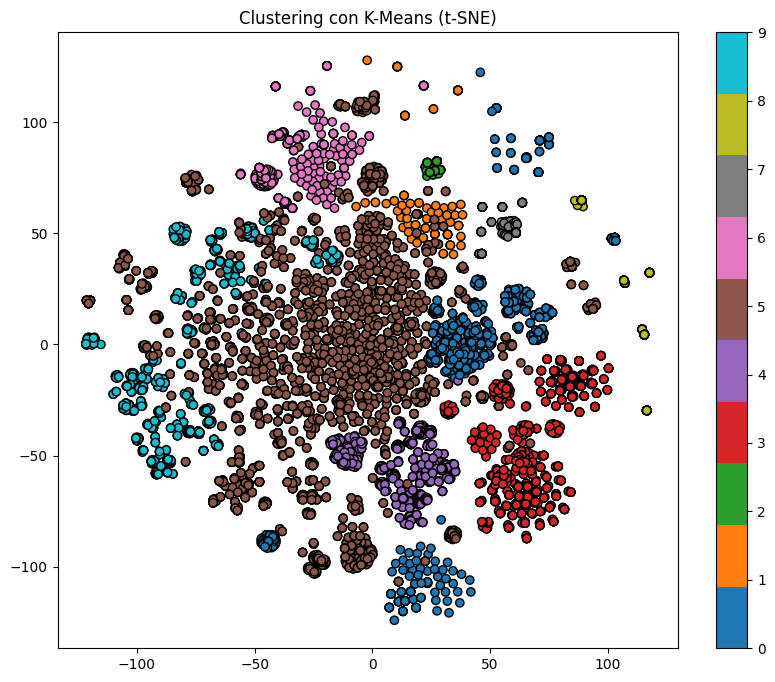
\includegraphics[width=0.7\linewidth]{imagenes/k-means-tf-idf-t-sne.png}
    \caption{Clustering con K-Means utilizando \gls{TF}-\gls{IDF} y \gls{t-SNE}}
    \label{fig:k-means-tf-idf-t-sne}
\end{figure}

\vspace{-3mm}

El resto de \textit{clusters}, como se ha indicado anteriormente, no contienen ninguna palabra que pueda estar asociada algún ataque:


\begin{mdframed}
\scriptsize
\begin{minted}{javascript}
Cluster 0: main, 09, 08, dnd, x11, received, events, debian, host, 47
Cluster 1: retries, ignoring, max, pam, sshd, service, devices, device, devel
Cluster 4: containerd, 05, info, io, msg, 2024, time, level, 02, v1
Cluster 5: service, target, pipewire, agent, device, entered, socket, starting
Cluster 6: session, uid, pam_unix, cron, root, user, opened, closed, sudo, lightdm
Cluster 7: supervising, processes, threads, users, 10, 12, 13, 11, 14, 15
Cluster 9: service, successfully, org, bus, pid, uid, deactivated, 1000, dbus
\end{minted}
\end{mdframed}

Comparando el resultado obtenido con \gls{TF}-\gls{IDF} en K-means y a continuación, con \textit{Count Vectorizer} en \gls{AHC} (Figura \ref{fig:k-means-count-vectorizer-t-sne}), se observa una ligera mejora, ya que la amplia mayoría de \textit{logs} asociados a ataques se agrupan en el \textit{cluster} dos, y el resto en el quinto y el séptimo.

\begin{mdframed}
\scriptsize
\begin{minted}{javascript}
Cluster 2: port, 172, 17, ssh2, password, failed, invalid, anonymous, user, root
Cluster 5: euid, ruser, logname, rhost, tty, ssh, authentication, uid, 172, 
failure
Cluster 7: pass, unknown, check, auth, sshd, pam_unix, user, device, devel,
failure
\end{minted}
\end{mdframed}

\begin{figure}[H]
    \centering
    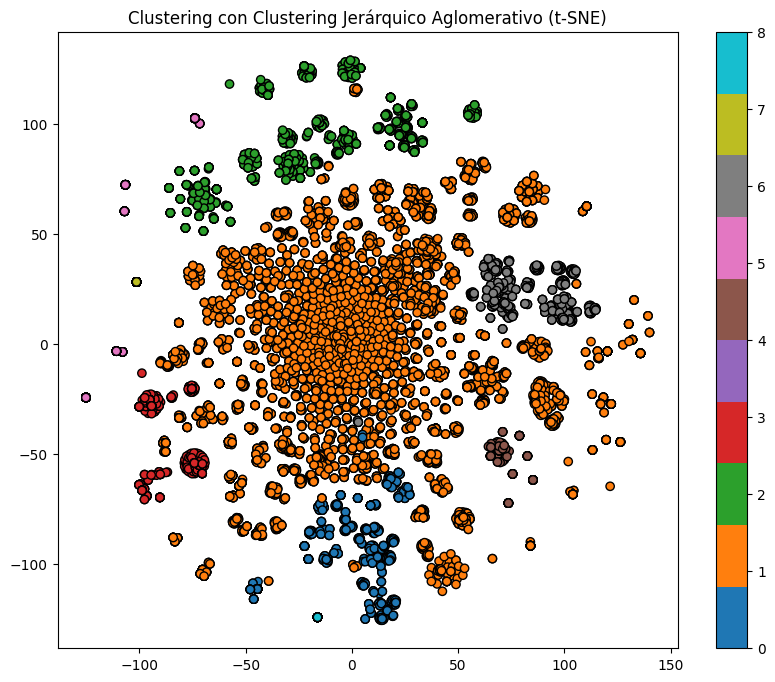
\includegraphics[width=0.7\linewidth]{imagenes/AHC-count-vectorizer-t-sne.png}
    \caption{Clustering con \gls{AHC} utilizando \textit{Count Vectorizer} y \gls{t-SNE}}
    \label{fig:k-means-count-vectorizer-t-sne}
\end{figure}

El hecho de que \gls{DBSCAN} haya tenido buenos resultados con \textit{Silhouette Score} y al mismo tiempo unos muy bajos en las otras dos métricas como se muestra en la Figura \ref{fig:dataset_01}, se debe a la gran cantidad de \textit{clusters} que tiene, de modo que reajustando sus parámetros podría mejorar el resultado en estas últimas. No obstante, se tendrá en cuenta este resultado para ver qué comportamiento presenta este algoritmo de \textit{clustering} en los demás conjuntos de datos.

\begin{figure}[H]
    \centering
    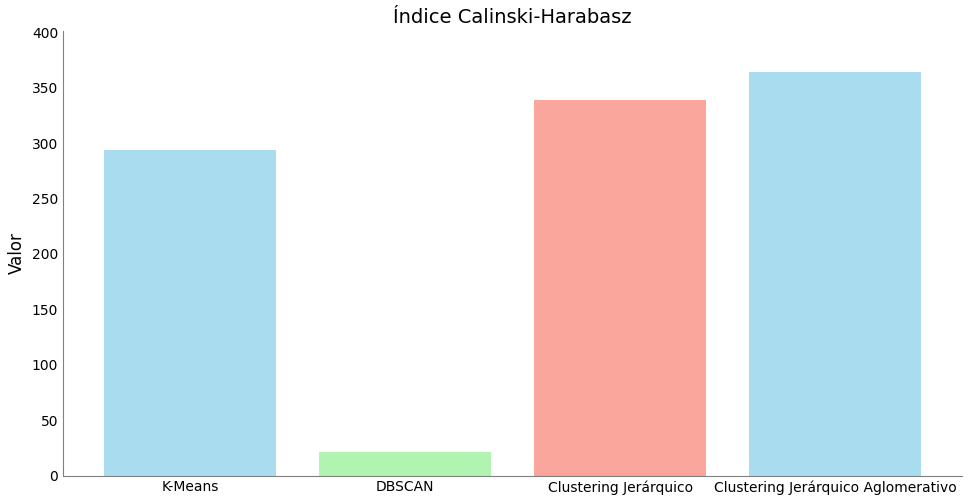
\includegraphics[width=0.8\linewidth]{imagenes/dataset_01_calinski.png}
    \caption{Resultados obtenidos en \textit{dataset} manual según índice de Calinski-Harabasz}
    \label{fig:dataset_01}
\end{figure}

En el caso del segundo conjunto de datos: \texttt{02\_linux-logs-2k.csv}, el cual contiene también eventos generados por \textit{syslog} en una máquina Linux del año 2016, se incluyen principalmente intentos de inicio de sesión fallidos. Al aplicar los cuatro algoritmos de \textit{clustering}, se han obtenido algunos resultados de interés. \\

Para el algoritmo \textit{K-means} se aplicó el Algoritmo del Codo, y se obtuvo un valor de codo cercano a k=4 tal y como se muestra en la Figura \ref{fig:metodo-codo-dataset-02}. En este caso el resultado es claro, por lo tanto ha sido necesario aproximar de nuevo el valor de \textit{k} por medio de Silhouette Score.

\begin{figure}[H]
    \centering
    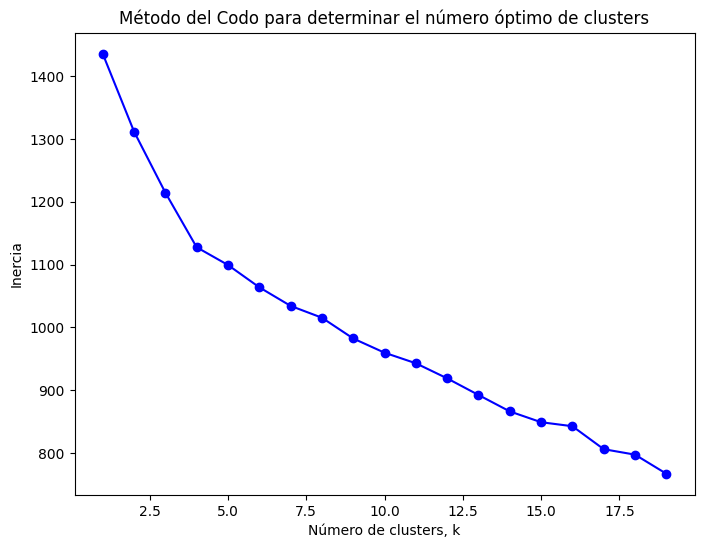
\includegraphics[width=0.7\linewidth]{imagenes/metodo-codo-dataset_02.png}
    \caption{Cálculo del método del codo para el \textit{dataset} \texttt{02\_linux-logs-2k.csv}}
    \label{fig:metodo-codo-dataset-02}
\end{figure}

\vspace{-2mm}

Utilizando ambas técnicas de reducción de dimensionalidad se obtienen unos resultados muy similares. Los \textit{logs} asociados a eventos críticos de seguridad se han podido agrupar en un mismo \textit{cluster}: el número uno.

\begin{figure}[H]
    \centering   
    \begin{minipage}{0.4\textwidth}
        \centering
        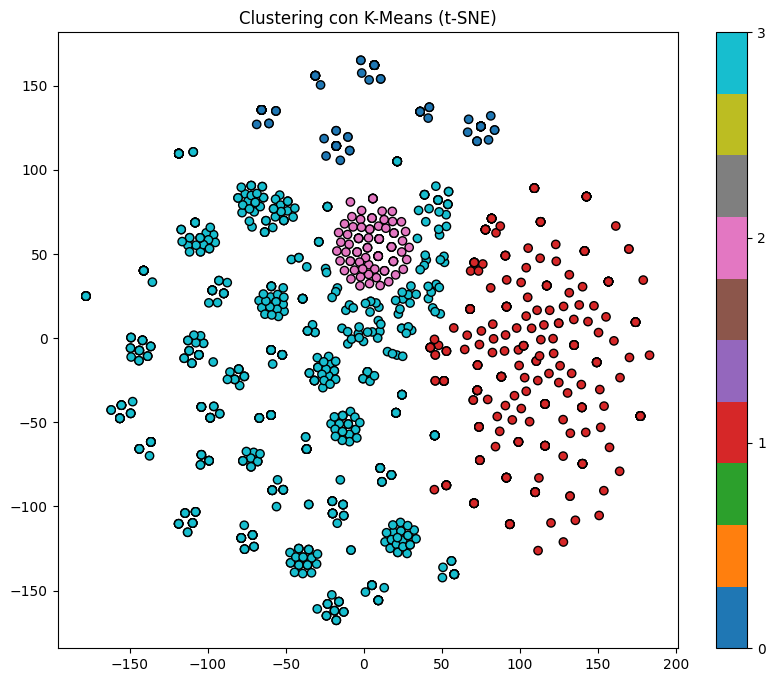
\includegraphics[width=\linewidth]{imagenes/dataset_02_k-means_t_sne_count_vectorizer.png}
        \caption{Clustering de \textit{Linux\_2k} con K-means utilizando \gls{TF}-\gls{IDF} y \gls{t-SNE}}
        \label{fig:dataset_02_k-means_tsne_tf_idf}
    \end{minipage}
    \hspace{0.1\textwidth}
    \begin{minipage}{0.4\textwidth}
        \centering
        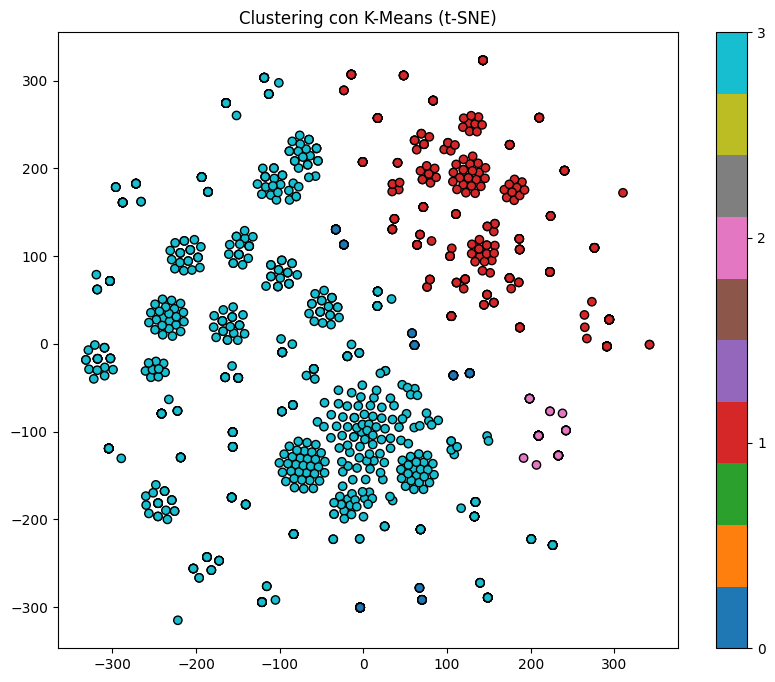
\includegraphics[width=\linewidth]{imagenes/dataset_02_k-means_tsne_tf_idf.png}
        \caption{Clustering de \textit{Linux\_2k} con K-means utilizando \textit{Count-Vectorizer} y \gls{t-SNE}}
        \label{fig:dataset_02_k-means_tsne_count_vectorizer}
    \end{minipage}
\end{figure}

En la Figura \ref{fig:dataset_02_k-means_tsne_tf_idf} se agrupan bajo el \textit{cluster} uno, al igual que en la Figura \ref{fig:dataset_02_k-means_tsne_count_vectorizer}. Además su contenido es equivalente:

\begin{mdframed}
\scriptsize
\begin{minted}{javascript}
Cluster 1: ruser, rhost, euid, logname, tty, failure, nodevssh, authentication, 
uid, root
\end{minted}
\end{mdframed}

Para realizar una comparativa con \textit{datasets} de eventos distintos a los de \textit{syslog} en Linux, se ha seleccionado el conjunto de datos asociado a un fragmento de 20000 líneas de \gls{HDFS}, generado en el año 2008. Los resultados obtenidos distan bastante con los anteriores, en primer lugar debido a que ha aumentado significativamente el volumen de datos \textit{clusterizados}, y en segundo lugar por la información recopilada por estos \textit{logs}, por tanto se presentan anomalías distintas, tal y como se muestra en la Figura \ref{fig:hdfs-ahc-t-sne} en el caso del algoritmo \gls{AHC}. Al aplicar el método del codo, se ha obtenido un valor óptimo de \textit{clusters} con \textit{k=13}.

\begin{figure}[H]
    \centering
    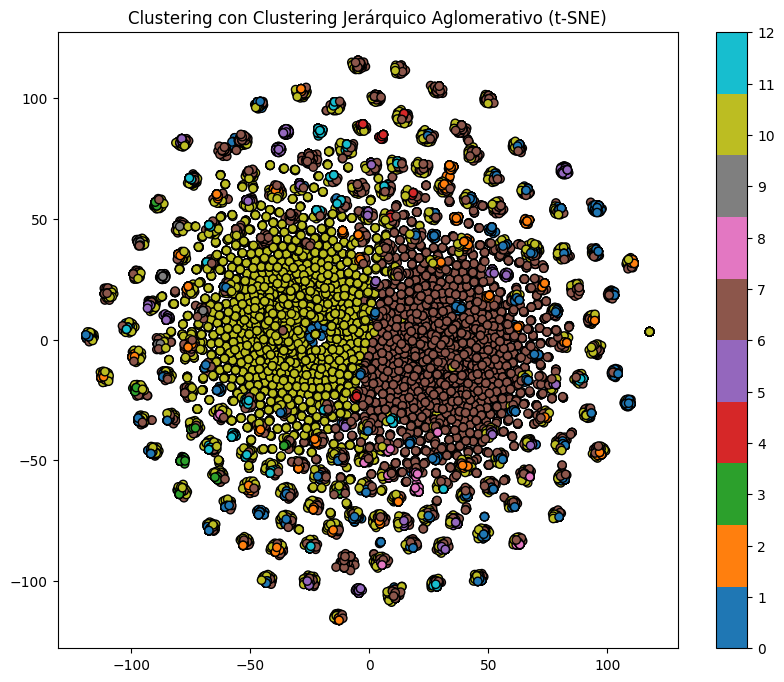
\includegraphics[width=0.8\linewidth]{imagenes/dataset_03_AHC_tf_idf.png}
    \caption{Clustering de \gls{HDFS} con \gls{AHC} utilizando \gls{TF}-\gls{IDF} y \gls{t-SNE}}
    \label{fig:hdfs-ahc-t-sne}
\end{figure}

En la Figura \ref{fig:hdfs-ahc-t-sne}, los principales \textit{clusters} son el siete y el diez. Cada uno de ellos hace referencia a operaciones críticas sobre grandes bloques de datos, como finalizar una transferencia. Sin embargo, no se aprecia ninguna operación que llegue a resultar de utilidad para detectar algún tipo de acción indeseada, por lo que se demuestra una vez más la vital importancia de que los \textit{logs} registren la información de la manera más clara posible en lenguaje natural, de modo que pueda ser clasificada de forma óptima por modelos de inteligencia artificial. Los \textit{logs} de \gls{HDFS} utilizan una terminología muy específica y ambigüa, que tendría que ser mapeada para poder facilitar al modelo su proceso de razonamiento y que pueda otorgar buenos resultados.

\begin{mdframed}
\scriptsize
\begin{minted}{javascript}
Cluster 7: terminating, block, updated, added, size, 67108864, 50010, 10, 251,250
Cluster 10: blk_, terminating, block, updated, added, 67108864, size, 50010, 10,25
\end{minted}
\end{mdframed}

En cuarto lugar, para \gls{BGL}, que se trata de un conjunto de datos del supercomputador de \gls{IBM} como se ha explicado en capítulos anteriores, se ha calculado un valor óptimo de \textit{k=4} \textit{clusters}. Este valor, al igual que en los ejemplos anteriores, se ha calculado a partir de aplicar el Algoritmo del Codo. En este caso se han agrupado en el cluster cero (azul) \textit{cluster} los eventos asociados a errores del \textit{Kernel}, como se puede observar en la Figura \ref{fig:dataset_04_umap}. 

\begin{figure}[H]
    \centering
    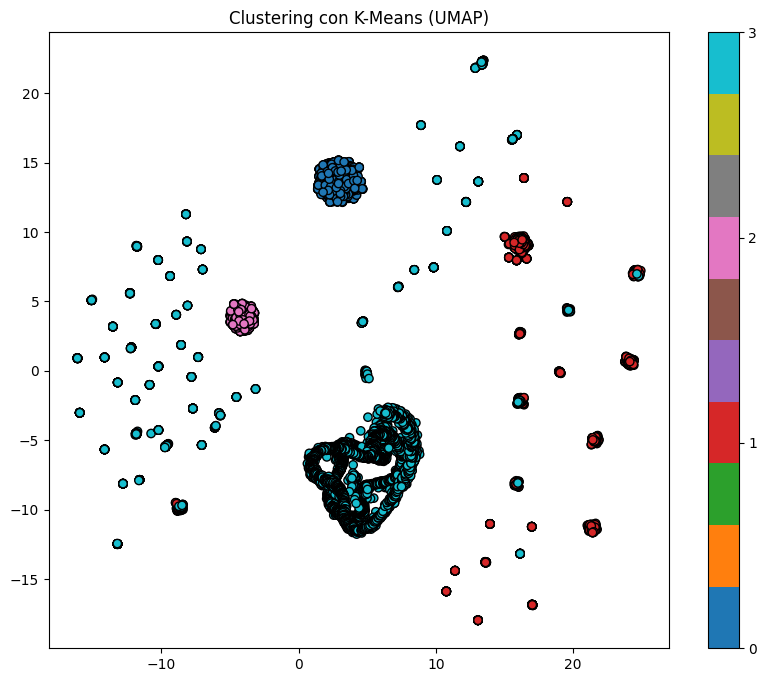
\includegraphics[width=0.6\linewidth]{imagenes/dataset_04_k-means-umap.png}
    \caption{Clustering de \gls{BGL} con K-means utilizando \gls{TF}-\gls{IDF} y \gls{UMAP}}
    \label{fig:dataset_04_umap}
\end{figure}

Se han obtenido unos resultados prácticamente equivalentes para el caso de los algoritmos de \textit{clustering} jerárquico y su variante aglomerativa. De los cuatro \textit{clusters}, se dividen varios tipos de alertas. Por un lado, en el grupo cero aquellas relacionados con errores del \textit{kernel} y la memoria caché. En el caso del \textit{cluster} uno, se agrupan problemas relacionados con excepciones y aliniamiento. Esto es positivo, ya que no simplemente se agrupan alertas en uno solo, sino que se fusionan en base a la tipología del error que ocasiona el evento.


\begin{mdframed}
\scriptsize
\begin{minted}{javascript}
Cluster 0: cache, instruction, parity, corrected, error, info, kernel, 35737, 
35717, 35716
Cluster 1: hummer, exceptions, double, alignment, kernel, info, 182, 162, 141, 142
Cluster 2: message, ciostream, control, socket, prefix, stream, read, 96, 116, 172
Cluster 3: info, core, generating, kernel, mask, ce, sym, 0x08, detected, ddr
\end{minted}
\end{mdframed}

En quinto lugar, el \textit{dataset} que ha sido generado de forma sintética, estaba formado de forma intencionada únicamente por alertas de seguridad asociadas a ataques de distinto ámbito. Si se obtienen unos buenos resultados, sería indicativo de que los algoritmos de \textit{clustering} responden de una forma adecuada cuando los conjuntos de datos de \textit{logs} son robustos, es decir, contienen eventos con una información completa y clara.

Los mejores resultados se han obtenido a través de la reducción de dimensionalidad con \textit{Count Vectorizer} y la vectorización de texto con \gls{t-SNE}. Como se observa en la Figura \ref{fig:dataset_05_count_vectorizer_t_sne}, se agrupan anomalías principalmente en los \textit{clusters} tres, uno y ocho. Su contenido difiere principalmente por los usuarios involucrados en el proceso de autenticación a un servidor \gls{SSH}. 

\begin{figure}[H]
    \centering
    \includegraphics[width=0.7\linewidth]{imagenes/dataset-sintético-t-sne-count-vectorizer.png}
    \caption{Clustering de \gls{AHC} en \textit{dataset} sintético con \textit{Count Vectorizer} y \gls{t-SNE}}
    \label{fig:dataset_05_count_vectorizer_t_sne}
\end{figure}

\vspace{-1mm}

En el siguiente fragmento de código se muestra el conjunto de palabras asociado a cada \textit{cluster}. El primero de ellos hace referencia a varios elementos como la desconexión de un suario y un intento de sesión fallida. El segundo (\textit{cluster 3}, se asocia con un \textit{login} inválido a causa de un usuario inexistente y otros exitosos pero de riesgo debido a que están relacionados con usuarios con permisos de administrador. Por último, el \textit{cluster} ocho contiene palabras relacionadas con un posible ataque de fuerza bruta que ha alcanzado un máximo de intentos de autenticación para un usuario \texttt{admin}. \\

\begin{mdframed}
\scriptsize
\begin{minted}{javascript}
Cluster 1: port, 168, 192, ssh2, failed, transfer, completed, user, disconnected
Cluster 3: logged, 168, 192, test, admin, guest, root, invalid_user, 51, 101
Cluster 8: exceeded, authentication, attempts, preauth, ssh2, port, 192, 168, 
test, admin
\end{minted}
\end{mdframed}


Una vez más, las métricas de Índice de Davies-Bouldin \cite{DaviesBouldin1979} e Índice de Calinski-Harabasz \cite{CalinskiHarabasz1974} otorgan una mayor puntuación a los algoritmos K-means, \gls{HC} y \gls{AHC}, mientras que \textit{Silhouette Score} da la valoración más positiva a \gls{DBSCAN}.

Finalmente, para el conjunto de datos \texttt{06\_auth-logs-20k.csv}, se ha calculado de nuevo mediante el Algoritmo del Codo el valor de \textit{k} para utilizarlo en los algoritmos jerárquicos y K-means, obteniendo un valor de 12. El tamaño original de este era de 47000 eventos de seguridad, sin embargo debido a las limitaciones de computación ha sido necesario tomar un fragmento de 20000.

Los resultados obtenidos han sido, en comparación con los \textit{datasets} generados tanto de forma manual como sintética, significativamente peores, tal y como puede observarse en la Figura \ref{fig:dataset_06}. 

\newpage

Esto se debe principalmente a que los eventos capturados en este fichero provienen del fichero \texttt{auth.log}, que únicamente almacena logs a sociados a intentos de inicio de sesión fallidos. Es por ello, que sería interesante tratar de otro modo el \textit{corpus} para que se realizara el \textit{clustering} en base a los usuarios que han llevado a cabo el proceso de autenticación.

\begin{figure}[H]
    \centering
    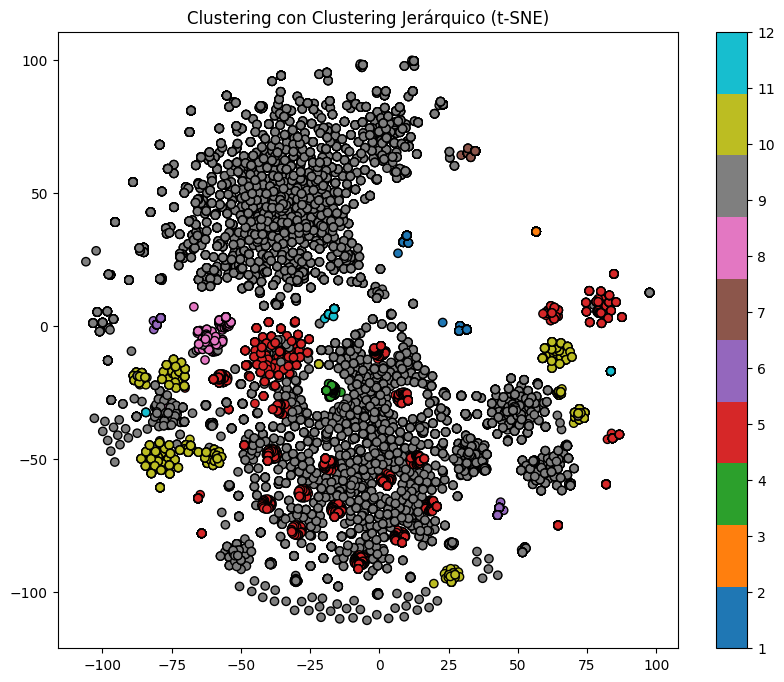
\includegraphics[width=0.675\linewidth]{imagenes/dataset_06_count_vectorizer_t-sne.png}
    \caption{Clustering de \gls{HC} en \texttt{06\_auth-logs-20k.csv} con \textit{Count Vectorizer} y \gls{t-SNE}}
    \label{fig:dataset_06}
\end{figure}

\vspace{-4mm}

Todas las gráficas anteriores que muestran los resultados de un análisis de \textit{clustering} después de aplicar alguna técnica de reducción de dimensionalidad se representan por los siguientes ejes:
\begin{itemize}
    \item \texttt{Eje X} (horizontal): Corresponde a la primera componente principal, que captura la dirección de máxima varianza de los datos, mostrando dónde los datos varían más.
    \item \texttt{Eje Y} (vertical): Corresponde a la segunda componente principal, que captura la siguiente dirección de máxima varianza, perpendicular a la primera. \\
\end{itemize}


En conclusión, los algoritmos de \textit{clustering} que mejor han respondido ante estos conjuntos de datos han sido, por amplia diferencia K-means y los algoritmos jerárquicos \gls{HC} y \gls{AHC}. En cuanto a la técnica de vectorización de texto que mejores prestaciones ha tenido en base a las métricas utilizadas ha sido \textit{Count Vectorizer}. Por último, la técnica de reducción de dimensionalidad que ha permitido graficar de forma más óptima los conjuntos de \textit{logs} ha sido \gls{t-SNE}. 

En la Figura \ref{fig:resultados-dataset-manual} pueden visualizarse los resultados obtenidos para el \textit{dataset} generado manualmente (\texttt{01\_linux-logs-9k.csv}) aplicando los distintos algoritmos de \textit{clustering} en base a las técnicas utilizadas para vectorización de texto y reducción de dimensionalidad. Además, en la Tabla \ref{tab:metricas} pueden consultarse los valores obtenidos en base a las tres métricas utilizadas y clasificados por algoritmo utilizado y técnica de vectorización de texto.

\newpage
  
\noindent \hspace{-11mm}
\begin{minipage}{\linewidth}
        \begin{figure}[H]
            \centering
            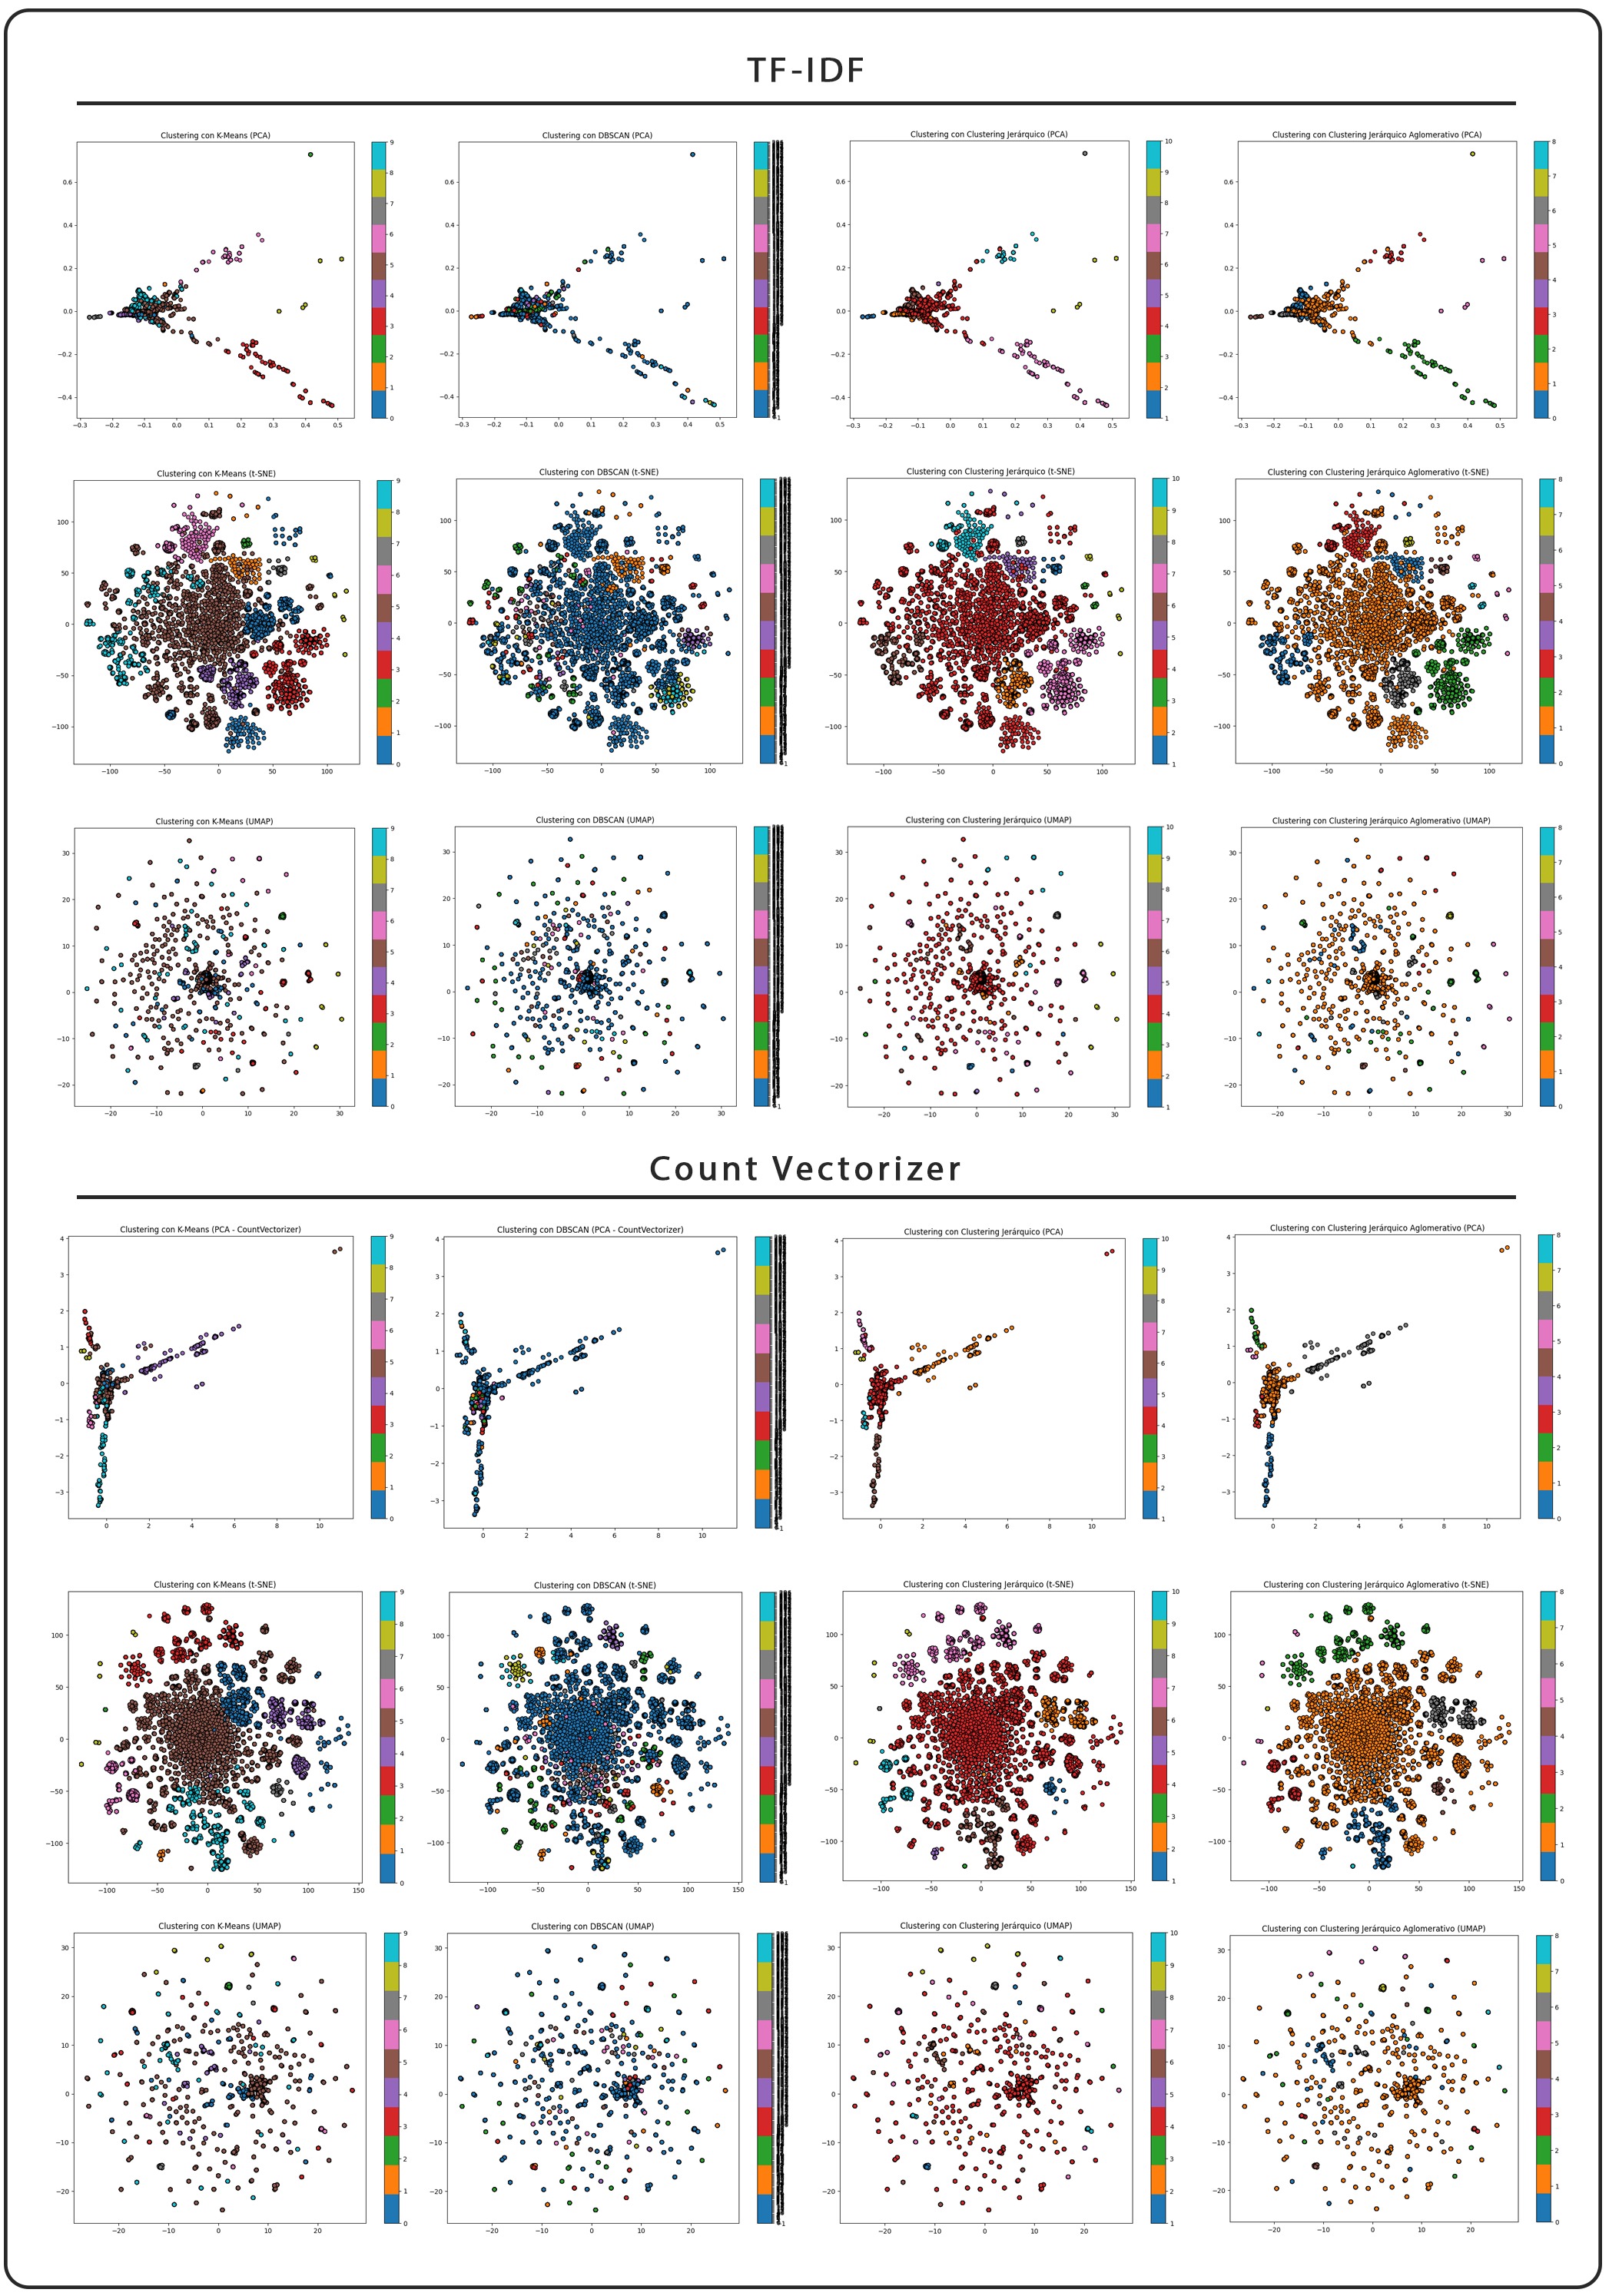
\includegraphics[width=1.2\linewidth, keepaspectratio]{imagenes/graficas-dataset-manual.png}
            \caption{Resultados del \textit{clustering} obtenidos en el \textit{Dataset} manual}
            \label{fig:resultados-dataset-manual}
        \end{figure}
\end{minipage}

\newpage
\thispagestyle{empty}

\begin{landscape}
    \noindent\hspace*{-3.1cm}
    \footnotesize
    \begin{tabularx}{2.1\textwidth}{|l|>{\hsize=1\hsize}X|X|X|X|X|X|X|X|X|}
    \rowcolor{graylight}
        \hline
        \multicolumn{2}{|l|}{\texttt{Métrica Utilizada}} & \multicolumn{4}{c|}{\texttt{TF-IDF}} & \multicolumn{4}{c|}{\texttt{CountVectorizer}} \\ \hline
        \texttt{Dataset} & \texttt{Número Eventos} & \texttt{K-means} & \texttt{DBSCAN} & \texttt{HC} & \texttt{AHC} & \texttt{K-means} & \texttt{DBSCAN} & \texttt{HC} & \texttt{AHC} \\ \hline
        \rowcolor{graylight} \multicolumn{10}{|c|}{\texttt{Silhouette Score}} \\ \hline
        \texttt{01\_linux-logs-9k.csv} & 8890 & 0,142565 & \textbf{0,327076} & 0,148059 & 0,138362 & 0,045752 & 0,223888 & 0,056558 & 0,047342    \\ \hline
        \texttt{02\_linux-logs-2k.csv} & 1546 & 0,186831 & \textbf{0,856451} & 0,186831 & 0,186831 & 0,120715 & 0,834370 & 0,120715 & 0,120715    \\ \hline
        \texttt{03\_HDFS-logs-20k.csv} & 20000 & 0,055194 & -0,01371 & 0,020737 & 0,018550 & \textbf{0,129202} & -0,10574 & 0,026898 & 0,024624   \\ \hline
        \texttt{04\_BGL-logs-20k.csv} & 20000 & 0,367028 & 0,476697 & 0,363458 & 0,363458 & 0,596589 & 0,345334 & \textbf{0,582639} & \textbf{0,582639}   \\ \hline
        \texttt{05\_Synthetic-logs-5k.csv} & 5000 & 0,183675 & \textbf{0,327810} & 0,168854 & 0,177956 & 0,166143 & 0,254842 & 0,172808 & 0,153171    \\ \hline
        \texttt{06\_auth-logs-20k.csv} & 20000 & 0,337545 & 0,661056 & 0,342969 & 0,342969 & 0,351366 & \textbf{0,645813} & 0,277735 & 0,277735  \\ \hline
        \rowcolor{graylight} \multicolumn{10}{|c|}{\texttt{Indice de Davies-Bouldin}} \\ \hline
        \texttt{01\_linux-logs-9k.csv} & 8890 & \textbf{3,160860} & 1,101850 & 2,215990 & 2,427580 & 2,543825 & 1,217092 & 1,697760 & 1,813962    \\ \hline
        \texttt{02\_linux-logs-2k.csv} & 1546 & \textbf{2,042738} & 1,040805 & \textbf{2,042738} & \textbf{2,042738} & 1,638323 & 0,840527 & 1,638323 & 1,638323   \\ \hline
        \texttt{03\_HDFS-logs-20k.csv} & 20000 & 3,914300 & 1,052135 & 5,081278 & \textbf{5,365123} & 2,195493 & 1,426535 & 3,877497 & 4,802849   \\ \hline
        \texttt{04\_BGL-logs-20k.csv} & 20000 & 1,830761 & 0,952598 & \textbf{1,883499} & \textbf{1,883499} & 0,728352 & 0,854809 & 0,759906 & 0,759906   \\ \hline
        \texttt{05\_Synthetic-logs-5k.csv} & 5000 & \textbf{2,471757} & 1,028901 & 2,254009 & 2,359428 & 1,789288 & 1,127338 & 1,673542 & 1,722449   \\ \hline
        \texttt{06\_auth-logs-20k.csv} & 20000 & \textbf{2,067445} & 1,035235 & 1,589178 & 1,589178 & 1,695114 & 0,982265 & 1,317203 & 1,317203   \\ \hline
        \rowcolor{graylight} \multicolumn{10}{|c|}{\texttt{Indice de Calinski-Harabaz}} \\ \hline
        \texttt{01\_linux-logs-9k.csv} & 8890 & 247,64400 & 24,20370 & 254,66300 & 267,61000 & 293,662881 & 21,363775 & 338,759653 & \textbf{364,631418}  \\ \hline
        \texttt{02\_linux-logs-2k.csv} & 1546 & 140,494849 & 156,210995 & 140,494849 & 140,494849 & 205,211041 & \textbf{235,150142} & 205,211041 & 205,211041   \\ \hline
        \texttt{03\_HDFS-logs-20k.csv} & 20000 & 254,81996 & 170,938375 & 173,080575 & 180,749527 & 1303,516335 & 10,251355 & 607,210643 & \textbf{664,011968}    \\ \hline
        \texttt{04\_BGL-logs-20k.csv} & 20000 & 4263,557621 & 159,093892 & 4176,9412 & 4176,9412 & \textbf{18712,75285} & 182,430667 & 17821,29833 & 17821,29833   \\ \hline
        \texttt{05\_Synthetic-logs-5k.csv} & 5000 & 249,890189 & 58,079644 & 255,864348 & 263,576459 & 530,687883 & 60,799303 & 554,721452 & \textbf{565,499024}  \\ \hline
        \texttt{06\_auth-logs-20k.csv} & 20000 & 1443,017509 & 112,332262 & 1431,08245 & 1431,08245 & \textbf{3297,852755} & 148,411853 & 2295,506274 & 2295,506274    \\ \hline
    \end{tabularx}
    \begin{table}[H]
        \centering
        \caption{Métricas obtenidas en los distintos conjuntos de datos}
        \label{tab:metricas}
    \end{table}
\end{landscape}

\newpage

% ********************************************************************

\section[Estudios previos para la detección de amenazas]{Análisis comparativo. Estudios previos para la detección de amenazas}

En la misma línea que este Trabajo de Fin de Grado, a lo largo de estos últimos años han emergido numerosas propuestas para la detección proactiva de actividades maliciosas por medio de técnicas que apliquen de un modo u otro inteligencia artificial. A lo largo de esta sección se abordarán las principales alternativas publicadas en distintas fuentes institucionales como \textit{Google Scholar}, \textit{Scopus} o \textit{Science Direct}. \\

% ********************************************************************

\subsubsection*{Primer caso de Estudio}

Comenzando por el artículo publicado por Kayhan et. al \cite{KAYHAN2023113928}, se propone el uso de \gls{UHAC} (\textit{Unsupervised hunting of anomalous commands}), que precisamente sigue el enfoque de detectar anomalías a través de conjuntos de datos no etiquetados en \gls{SIEM}s mediante \textit{clustering}. En concreto, hace uso de \gls{TF}-\gls{IDF} para la creación de la matriz de características y \gls{DBSCAN} para el \textit{clustering}. Además, emplea una función de pérdida personalizada que le permite manejar de forma adecuada los pesos binarios\footnotemark. Los comandos se van ordenando en base a su error de reconstrucción, de modo que los errores más altos son indicativo de una mayor probabilidad de la existencia de anomalías. 

\footnotetext{Pesos que indican la presencia (1) o ausencia (0) de características específicas en los comandos.}

En esta investigación, se hizo uso de \gls{OC-SVM} (\textit{One-Class Support Vector Machine}), que se trata de una técnica de clasificación empleada para la detección de anomalías, especialmente efectiva en contextos donde los datos etiquetados son escasos o inexistentes. Este construye un modelo a partir de un conjunto de datos no etiquetados, diferenciando entre patrones normales y aquellos que se consideran anomalías, mediante la maximización del margen de separación en un espacio de características transformado.

\subsubsection*{Segundo caso de Estudio}

En el \textit{paper} publicado por Tendikov et. al \cite{TENDIKOV2024102254}, se lleva a cabo una evaluación de la efectividad de distintos modelos de \gls{ML} con el propósito principal de detectar intrusiones en redes. Para ello, se levó a cabo una recopilación datos de máquinas virtuales Windows capturados por un \gls{SIEM}, más concretamente ataques web procedentes del \textit{dataset} CICIDS2017 \cite{sharafaldin2018toward}. En cuanto a las técnicas de \textit{clustering} utilizadas, se incluyen \textit{Random Forest} y K-means, así como técnicas de vectorización de texto como \gls{TF}-\gls{IDF} y de reducción de dimensionalidad como \gls{PCA} y \gls{t-SNE}. Por último, para medir los resultados obtenidos se hizo uso de la métrica F1 Score, mediante la cual se obtuvo un 0,97 utilizando \textit{Random Forest}.

\newpage

% ********************************************************************

\subsubsection*{Tercer caso de Estudio}
% https://link.springer.com/book/10.1007/978-3-030-74450-2 
En tercer lugar, en el libro de Skopik et. Al \cite{skopik2021smart}, se lleva a cabo una clasificación de los tipos de anomalías que pueden llegar a ser detectadas a través de algoritmos de \textit{clustering}. Entre estas destacan:

\begin{itemize}
\item \texttt{Outliers}\label{outliers}: también conocidos como valores atípicos, son líneas de registro individuales que no coinciden con ninguna de las plantillas existentes o son disímiles a todos los \textit{clusters} identificados que representan el comportamiento normal del sistema. Un ejemplo podría ser un mensaje de error en un archivo de registro que generalmente solo contiene mensajes informativos y de depuración. \\
\item \texttt{Anomalías de Frecuencia}: son eventos de registro que aparecen con una frecuencia inesperadamente alta o baja durante un intervalo de tiempo dado. Esto incluye casos donde los componentes dejan de registrar eventos o la detección de ataques que implican la ejecución de muchos eventos, como los escaneos de vulnerabilidades. \\
\item \texttt{Anomalías de Correlación}: eventos que se espera que ocurran en pares o grupos pero no lo hacen. Un claro ejemplo serían anomalías de coocurrencia y de implicación, es decir, aquellos eventos que deberían implicar la ocurrencia de otros. \\
\item \texttt{Anomalías de Tiempo entre Llegadas}: Causadas por intervalos de tiempo desviados entre la ocurrencia de \textit{logs}. Estas están relacionadas con las de correlación y pueden proporcionar capacidades de detección adicionales, por ejemplo, si un evento esperado no ocurre dentro de una ventana de tiempo específica. \\
\item \texttt{Anomalías de Secuencia}: son provocadas por eventos faltantes o adicionales, así como por órdenes desviadas en secuencias de eventos de registro que se esperan ocurran en ciertos patrones.
\end{itemize}

Estos tipos de anomalías pueden ser detectadas o apoyadas por técnicas de \textit{clustering} tanto estáticas como dinámicas, dependiendo del tipo específico de anomalía. Los \textit{outliers} pueden ser identificados mediante algoritmos de \textit{clustering} estático, mientras que las demás anomalías requieren técnicas de \textit{clustering} dinámico y análisis estadístico para detectar violaciones en las correlaciones esperadas.

% ********************************************************************

\subsubsection*{Cuarto caso de Estudio}
% https://ieeexplore.ieee.org/document/10306968
Otro caso digno de análisis es el del \textit{paper} publicado por Tharunika et. al \cite{10306968}, titulado \textit{Detection and Prevention of Advanced Persistent Threat (APT) Activities in Heterogeneous Networks using \gls{SIEM} and Deep Learning}. En este se comenta el uso de modelos de \gls{ML} y \gls{DL} para la detección y prevención de anomalías de red en \gls{SIEM}s. Para ello, se hace uso de la arquitectura de la Figura \ref{fig:architecture-diagram}.

\begin{figure}[H]
    \centering
    \includegraphics[width=1\linewidth]{imagenes/architecture-diagram-v3.png}
    \caption{Diagrama de la arquitectura propuesta por Tharunika et. al \cite{10306968}}
    \label{fig:architecture-diagram}
\end{figure}

Tal y como se puede observar, tras el proceso de recopilación del conjunto de datos, se lleva a cabo una fase de preprocesamiento en la que se eliminan \gls{NaN}s, líneas duplicadas y \textit{outliers} \ref{outliers}. A continuación se lleva a cabo el \textit{encoding} y la selección de características. Seguidamente, se hace uso de técnicas de reducción de la dimensionalidad como \gls{PCA} y \gls{SVD}. Se emplean además algoritmos de \textit{clustering} como \gls{SMOTE} o K-means. Finalmente se lleva a cabo la generación de modelos, más concretamente se utilizan los siguientes:

\begin{itemize}
    \item Modelos de \gls{ML}: \gls{KNN}, \gls{SVM}, \textit{Random Forest} y Árboles de decisión.
    \item Modelos de \gls{DL}: \gls{ANN} y \gls{LSTM}.
\end{itemize}

Por medio del uso de estos modelos, se trataba de detectar si un \textit{log} o conjunto de \textit{logs} estaban asociados a un ataque de tipo \gls{DDoS} o si eran benignos. Para evaluar los resultados obtenidos se hizo uso de cuatro métricas distintas. Estas métricas fueron: \textit{Precission}, \textit{Recall}, \textit{F1-Score} y \textit{Accuracy}. Según las tablas obtenidas se obtuvieron unos resultados muy positivos, lo cual demuestra de nuevo la importancia de llevar a cabo un buen preprocesamiento de los conjuntos de datos de \textit{logs}.

% ********************************************************************

\subsubsection*{Quinto caso de Estudio}
% https://ieeexplore.ieee.org/stamp/stamp.jsp?tp=&arnumber=9614848
En línea con los estudios previos, el trabajo realizado por Datta et al. \cite{9614848} en su artículo titulado \textit{Real-time Threat Detection in \gls{UEBA} using Unsupervised Learning Algorithms} se enfoca en la detección de amenazas en tiempo real mediante el uso de algoritmos de aprendizaje no supervisado en el análisis del comportamiento de usuarios y entidades (\gls{UEBA}). En este estudio, se comparan cuatro algoritmos de \textit{clustering} no supervisados para detectar amenazas internas de manera eficiente.

Para la reducción de dimensionalidad, se utilizó el \gls{PCA}, permitiendo reducir las características del conjunto de datos a las más relevantes. En cuanto a las técnicas de preprocesamiento incluyeron \textit{One-Hot Encoding} para transformar datos categóricos en formato binario, estandarización para ajustar los valores de los datos, y la eliminación de duplicados y valores atípicos y así mejorar la calidad del conjunto de datos.

\newpage

Los modelos de \textit{Machine Learning} utilizados fueron:
\begin{itemize}
    \item \texttt{K-Means} (\ref{k-means})
    \item \texttt{\gls{AHC}} (\ref{dbscan})
    \item \texttt{\gls{DBSCAN}} (\ref{AHC})
    \item \texttt{\gls{GMM} (\textit{Gaussian Mixture Model})}: este es un modelo probabilístico que asume la existencia de un número finito de distribuciones Gaussianas, cada una representando un cluster. \\
\end{itemize}

Para evaluar el rendimiento de los algoritmos utilizados, se emplearon las mismas métricas que se han empleado para este Trabajo de Fin de Grado, es decir, Silhouette Score, índice de Calinski-Harabasz e Índice de Davies-Bouldin. Los resultados obtenidos en esta investigación fueron los mostrados en la Tabla \ref{tab:ueba-results}.

\begin{table}[H]
\centering
\footnotesize
\begin{tabularx}{\textwidth}{|X|X|X|X|}
\hline
\rowcolor{graylight} \texttt{Modelo} & \texttt{Silhouette Score} & \texttt{Calinski-Harabasz} & \texttt{Davies-Bouldin} \\ \hline
K-Means & 0.2372 & 887.8355 & 1.2291 \\ \hline
Agglomerative Clustering & 0.2291 & 718.8155 & 1.4191 \\ \hline
DBSCAN & 0.3782 & 345.2103 & 2.2108 \\ \hline
Gaussian Mixture Model (GMM) & 0.0697 & 191.3066 & 2.4507 \\ \hline
\end{tabularx}
\caption{Resultados obtenidos por Datta et al. \cite{9614848} empleando algoritmos de \textit{clustering} para la detección de amenazas}
\label{tab:ueba-results}
\end{table}

De este estudio se concluye que los algoritmos K-Means y \textit{Agglomerative Clustering} fueron los más eficientes para la detección de amenazas internas. Una vez más, se prueba que funcionan los métodos de \textit{clustering} no supervisados de cara a la detección de comportamientos anómalos en entornos de ciberseguridad. \\

% https://www.frontiersin.org/articles/10.3389/fdata.2024.1375818/full
Otro artículo estrechamente relacionado con este, es el de Artioli et al. \cite{artioli2024comprehensive}, en el cual se lleva a cabo una investigación exhaustiva sobre algoritmos de \textit{clustering} tanto tradicionales como emergentes aplicados a la \gls{UEBA}. En este estudio, se abordan diferentes contextos de aplicación y se consideran múltiples escenarios de interacción usuario-entidad. 

Artioli et al. comparan quince algoritmos de \textit{clustering} en tres conjuntos de datos diferentes, en los que destaca principalmente el rendimiento prometedor de \gls{HDBSCAN} y \gls{DenMune} en el conjunto de datos de comportamiento \gls{CERT}, generando grupos con una densidad muy cercana al número de usuarios.


% ********************************************************************

\subsubsection*{Sexto caso de Estudio}

En contraste con los casos de estudio anteriores, se ha tenido en cuenta el desarrollo de un \gls{LLM} orientado a ciberseguridad llamado \texttt{0dai} \cite{Navarrete2024}. A lo largo del año 2023 y este 2024, ha ido optimizándose y mejorando su capacidad de resolución de actividades relacionadas con el \textit{hacking} ético y la ciberseguridad. 0dai, además del uso genérico de \gls{LLM}s como \texttt{ \gls{GPT}} \cite{10500411} o \texttt{\gls{Gemini}} \cite{imran2024google}, propone el uso de agentes capaces de llevar a cabo ejercicios de \textit{pentesting} en hasta 15 minutos.

A diferencia de otros \textit{large model languages}, este no solo evita las limitaciones convencionales de su uso para actividades relacionadas con el \textit{hacking}, sino que está mejorado para implementar \textit{scripts} que utilicen herramientas de seguridad comunes e incluso implementar \textit{malware}. 

Además, \texttt{0dai} ha ido adquirido diversas funcionalidades adicionales. Ahora permite la integración con \gls{IDS}s y \gls{EDR}s, herramientas directamente relacionadas con un \gls{SIEM}. También ofrece acceso a una \textit{\gls{API} key} que permite usar el modelo de forma más personalizada, y ha logrado la integración con más de 50 herramientas de ciberseguridad. 

La reciente actualización \texttt{0dai} v2.0 incluye un modelo con 50 mil millones de parámetros y un sistema de registro para el \gls{FS}. Entre las herramientas utilizadas por sus usuarios se encuentran la implementación de \textit{bypass} de \textit{Cloudflare}, la herramienta Auto-\gls{XSS} para detectar vulnerabilidades \gls{XSS}, y mejoras en herramientas de \gls{OSINT} para buscar contraseñas y datos en brechas de seguridad.

Más allá de la ética relacionada con el uso que se le puede dar a este tipo de soluciones tecnológicas, pueden surgir múltiples soluciones que hasta ahora no se habían llevado a cabo. En base a una reunión con su entonces director de tecnología Luis Javier Navarrete, el pasado 8 de junio, se comentó que una de estas soluciones sería la creación de \textit{datasets} sintéticos a partir de agentes preparados con una serie de instrucciones muy específicas, de modo que se formaran conjuntos de datos verdaderamente útiles para entrenar modelos capaces de detectar anomalías de seguridad en distintos sistemas como Linux. 

Sin embargo, podría ser de mayor utilidad cambiar el enfoque de la metodología utilizada para la detección de vectores de ataque en este tipo de sistemas, de modo que se prepararan conjuntos de datos completamente etiquetados y que contuvieran información adicional, como mapear para cada \textit{log} si existe algún tipo de riesgo o no, o asignarle un potencial tipo de ataque (p.e. \gls{DDoS} o fuerza bruta al \textit{login} de algún servicio).

% ********************************************************************

% https://www.researchgate.net/profile/Omar-Al-Sanjary/publication/343408460_Comparison_and_Detection_Analysis_of_Network_Traffic_Datasets_Using_K-Means_Clustering_Algorithm/links/5f9977a9299bf1b53e4bb7df/Comparison-and-Detection-Analysis-of-Network-Traffic-Datasets-Using-K-Means-Clustering-Algorithm.pdf

\section{Sinergias e integración con sistemas \gls{SIEM}}
% https://www.mdpi.com/2076-3417/13/11/6610 

En el contexto de la amenaza constante por parte de los cibercriminales y ciberterroristas, la integración de la \gls{IA} con sistemas \gls{SIEM} es crucial para la detectar de forma efectiva incidentes y dar respuesta a estos en el menor tiempo posible. Según Ban et al.\cite{bantao2023}, los \gls{SIEM}s modernos deben abordar con diversos problemas, como es el caso de la fatiga de alertas, que puede llegar a resolverse mediante el uso de técnicas avanzadas de \gls{ML} y visualización de datos en tiempo real.

\vspace{-2mm}

\subsection{Beneficios de la integración}

La integración con sistemas \gls{SIEM} ya está proporcionando múltiples beneficios que pueden ser ampliados, entre ellos destacan:

\begin{itemize}
    \item Centralización de datos: la consolidación de \textit{logs} y eventos de seguridad en una plataforma centralizada facilita su análisis y correlación a los analistas de seguridad.

    \item Automatización de respuestas: Los \gls{SIEM}s pueden incorporar capacidades de \gls{SOAR} para automatizar tareas de respuesta a incidentes, mejorando la eficiencia operativa. 
    
    \item Reducción de falsos positivos: utilizando algoritmos de aprendizaje no supervisado o supervisado, como \gls{IWSVM} (\textit{Instance-Weighted Support Vector Machine}), propuesto por Ban et al.\cite{bantao2023}\footnotemark, es posible filtrar alertas irrelevantes y priorizar incidentes críticos.  
\end{itemize}

\footnotetext{\gls{IWSVM} es una mejora del \gls{SVM} tradicional que asigna diferentes pesos a las instancias basándose en su importancia, mejorando el rendimiento en conjuntos de datos desbalanceados.}

\vspace{-2mm}

\subsection{Desafíos y soluciones}

Uno de los mayores desafíos en la gestión de eventos de seguridad actualmente es la cantidad abrumadora de alertas generadas diariamente. Como se menciona en el trabajo de Ban et al.\cite{bantao2023}, se propuso un marco de \gls{SIEM} de próxima generación que integra capacidades avanzadas de \gls{SOAR} y utiliza una estrategia de \gls{DAC} para mitigar el impacto de las alertas de baja calidad.

A pesar de la funcionalidad que ofrecen los \gls{SIEM}s, estos presentan un cuello de botella con respecto a la toma de determinadas decisiones. Actualmente, en muchos casos es necesario que un profesional determine manualmente si hay algún tipo de intento de intrusión maliciosa, si hay un falso positivo o si simplemente no hay actividad inusual. Por lo tanto, a pesar de que la intervención humana seguirá siendo necesaria, la automatización de múltiples tareas permitirá que lso analistas inviertan su tiempo únicamente en decisiones críticas e \gls{I+D}. \\

La integración propuesta en este Trabajo de Fin de Grado implica la adopción por parte de un \gls{SIEM} de técnicas de \gls{ML} y visualización avanzada de los datos, con el principal propósito de mejorar la detección y respuesta a incidentes de seguridad. Entre estas técnicas, se propone especialmente utilizar algoritmos de \textit{clustering} como K-means y \gls{AHC}, ya que permiten una clasificación mucho más precisa que otras como \gls{DBSCAN} según los resultados obtenidos.

De tal modo, se conseguirá una sinergia con sistemas \gls{SIEM} que permitirá no solo la centralización y correlación de datos, sino también la automatización de tareas propias de un analista, así como la reducción de falsos positivos. En conclusión, los \gls{SIEM}s han sido desarrollados para ayudar a los administradores, no a sustituir su trabajo, y a facilitar el diseño de políticas de seguridad y la gestión de eventos con la mayor celeridad posible, aumentando su efectividad frente métricas como el \gls{MTTD} y \gls{MTTR}.

